\documentclass[10pt,a4paper]{article}
\usepackage[utf8]{inputenc}
\usepackage{amsmath}
\usepackage{amsfonts}
\usepackage{amssymb}
\usepackage{float}
\newcommand\tab[1][1cm]{\hspace*{#1}}
\usepackage{graphicx}
\usepackage{scrextend}
\usepackage{wrapfig}
\usepackage{enumitem}
\author{Konrad Cybulski, Julian Kardis, Matteo Batelic}
\title{Understanding Trends in Global Terrorism}
\begin{document}
\begin{titlepage}
    \begin{center}
        \vspace*{1cm}
        
        \LARGE
        \textbf{Understanding Trends in Global Terrorism}
        
        \vspace{4cm}
        
		\Large 
        
        \textbf{Konrad Cybulski, Julian Kardis, Matteo Batelic}
        
        
        \LARGE
        \vspace{2cm}

        
        
        \vfill
        
        
        
        Final report \\
        FIT2083 Research Project
        
        
        
\includegraphics[width=0.4\textwidth]{monash-university-logo.png}
              
        
        \large
        Faculty of Information Technology\\
        Monash University\\
        Australia\\
        24/10/2016
        
    \end{center}
\end{titlepage}

\pagebreak
\tableofcontents
\pagebreak

\section{Abstract} 

\section{Introduction} 
Terrorism is vast and complicated, being caused and provoked by numerous reasons.  This exploratory study aims to understand broad trends in global and country specific reigens. Utilising the ‘Global Terrorism Database’ from (START, 2016) consisting of ‘More than 150,000 terrorist attacks worldwide’ from 1970 to 2015 we aim to understand trends in countries with high rates of terrorism, methods of attacks, understanding rates of success in terror attacks and by utilising a count of both total and terrorism specific  articles produced by The New York Times newspaper we aim to answer if the recent influx of news articles due to the new accessibility of news has an effect on terrorism trends in America.

\pagebreak


	\section{Background}
		\subsection{The issues in terrorism research}
The scientific study of terrorism is plagued by three common issues throughout the literature.
			\subsubsection{Issue One: No universal agreement on a single definition of terrorism}
A common issue in the scientific study of terrorism is that there is no universal agreement on a single definition of terrorism (Charters, 1989). This lack of a common definition makes conveying sophisticated and nuanced ideas on terrorism difficult at best, as the definition of terrorism being used often depends upon the perspective the user is taking (Hill, 2016).  A clear example of this can be seen within the different agencies of the US government, many of which use different definitions of terrorism dependent of the departments priorities. \\\\

The US Department of State defines terrorism as “…means premeditated, politically motivated violence perpetrated against noncombatant targets by subnational groups or clandestine agents” (22 U.S Code) which focuses on politically motivated acts behind terrorism.  \\\\

The US Federal Emergency Management Agency defines terrorism as “…the use of force or violence against persons or property in violation of the criminal laws of the United States for purposes of intimidation, coercion, or ransom.” (FEMA, 2013), which is a focus on the criminal acts of terrorism.\\\\ 

The Federal Bureau of Investigations defines terrorism as “The unlawful use of force or violence against persons or property to intimidate or coerce a government, the civilian population, or any segment thereof, in furtherance of political or social objectives.” (FBI, 2002) which encompasses political, criminal and social aspects of terrorism. \\\\

There are also different definitions used by the U.S Department of Defense (DoD, 2010), the U.S Army Manual (U.S Army, 2001), and the U.S Congress (18 U.S Code), all of which focus on the different priorities of each department/branch of government. \\\\

For purpose of this study, the definition used is the same as the definition used by START. START defines terrorism as “Acts by non-state actors involving the threatened or actual use of illegal force or violence to obtain a political, economic, religious, or social goal through fear, coercion, or intimidation “ (START, 2016). 


			\subsubsection{Issue Two: A lack of objective data on terrorism}

The second common issue is a lack of objective data on terrorism (Silke, 2008). This is driven, at least in part, by the lack of a common definition of terrorism. But there are also other contributing factors, due to terrorism being a furtive activity by nature. \\\\

Terrorists are unlikely to report their activities, and in the rare cases they do, are usually doing so to drive factually dubious propaganda (Merari, 2007).  This is compounded by the fact many targets of terrorist attacks are governments, businesses or organizations. Frequently these targets are not interested in providing objective data about the attack due to not wanting to be perceived as vulnerable, not wanting to validate terrorist grievances or wanting to drive their own agenda (Lafree \& Dugan, 2007).\\\\



			\subsubsection{Issue Three: A lack of research to build upon}
Research on terrorism is not as widespread in relation to similar fields, such as criminology (LaFree \& Dugan, How does studying terrorism compare to studying crime?, 2004). The research has largely depended on a small pool of active researchers, and suffers from a distinct lack of collaborative research (Silke, 2008). Although since 9/11, papers in the field of terrorism have tripled, terrorism research is still lagging behind other similar fields of research (Sheehan, 2012).

		\subsection{Addressing the three common issues}
START has attempted to deal with these common issues by introducing several assumptions into their database.\\\\

For tackling the issue of lack of a common definition for terrorism, START have used modular criteria for their data, where an attack must meet several listed criteria (START, 2016). This rule is an attempt to address the lack of a universal definition for terrorism by allowing the components of several commonly used definitions to be used in conjunction.  START has not to included state sponsored terrorism and advises that due to a lack of a universal definition of insurgency (must like terrorism), that the database cannot be used for accurately modelling data based on insurgency. (START GTD, 2017).\\\\

For tackling the issue of objective data, START have decide to rely only on media reported incidents that meet their criteria rules for the definition of terrorism. START includes failed attacks but have decided to leave out failed or foiled plots, due to their underreporting (START, 2016). \\\\

In addressing the issue of lack of researchers and collaborative research in the field of terrorism, START have made their data set an open source endeavor. The problem introduced by this is that the database accuracy is dependent on the accuracy of media reports, and may be biased in favor of the most newsworthy forms of terrorism (START GTD, 2017).

\subsection{Methodological Issues with the GTD}

The data collection methods of the GTD have shifted over the years causing some inconsistencies within the data (START, 2016). This in part is explained by the fact that the groups collecting the data have changed, as well as an extended period of inactivity in the collection of data (LaFree, Dugan, \& Scott, 2006).
\\\\

\textbf{1993}\\\\
The entire year of 1993 is missing due to a clerical error (LaFree, Dugan, \& Scott, 2006).\\\\

\textbf{1997 - 2008}\\\\
The GTD data collection was discontinued between 1997 to 2008. It is for this reason there is a decline in data between 1998 and 2008. All records between this period were collected retroactively (LaFree, 2010).
\\\\

\textbf{2012 - Present}\\\\
Since 2007, the GTD has been funded by the Homeland of Security, with very little change to their methodology. However, in 2012 they were also jointly funded by the U.S State Department and moved base of operations to the University of Maryland, where they began to handle data collection locally, instead of through vendors (START, 2016). This change created a spike in the frequency of suicide attacks between 2011 and 2012 that was not observant in similar databases, such as Chicago Project on Security and Terrorism’s Suicide Attack Database (CPOST, 2016).
\\\\
\begin{center}
\begin{figure}[h!]
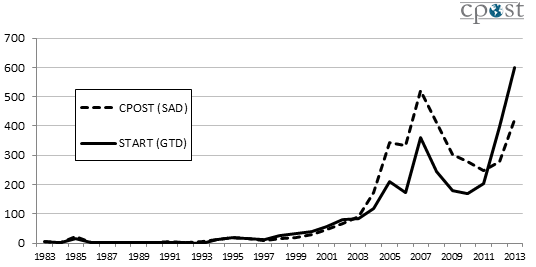
\includegraphics[width=0.9\textwidth]{backgroundpic1.png}
\caption{Comparison of terrorist suicide attacks between CPOST’s Suicide Attack Database and START’s Global Terrorism Database. The START database shows a statistically significant growth difference between 2011 and 2012}
\end{figure}
\end{center}

START has drawn criticism and been accused of politicizing their data (Pape, Kevin, Bauer, \& Jenkins, 2014). START dispute this, and cite their change from vendor based data collection to local based data collection as the reason for this increase in attacks in their data. (START GTD, 2017)

\subsection{START’s response to criticism }

In response to these issue, START has publicly stated that differences in trends before and after 1997, before and after 2008, and before and after 2012, can be, at least partially contributed to their data collection methodologies. START recommend any research using GTD data should adjust for these differences (START GTD, 2017).
\\\\
\begin{center}
\begin{figure}[h!]
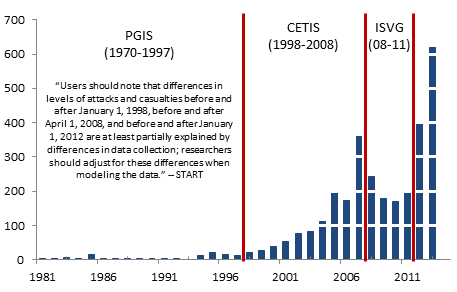
\includegraphics[width=0.9\textwidth]{backgroundpic2.png}
\caption{Critical methodology changes in the GTD. 
The graph shows terrorist attacks per year extracted from the GTD. The years data gathering methodology were changed are indicated by the red lines and labeled with  the organization responsible for the gathering of data for the GTD at the time.
}
\end{figure}
\end{center}

\newpage



\section{Method}
\subsection{Data}
The database used in this investigation comes from the Global Terrorism Database (GTD) (START, 2016) with 156,749 listings of successful and failed terrorist attacks around the world between 1970 and 2015. With additionally 137 variables including date, country, latitude/longitude, number of perpetrators, number of deaths as a result of the attack, number of injuries, method of attack (bombing, armed assault, etc.) as well as many others. Due to the extensive nature of the database, this investigation aims to understand trends in a select number of these variables. These variables include attack types, deaths, number of attacks, number of successful attacks, and country of attack. In order to understand country specific and global trends in terrorism, the data will be explored not only as a whole, but as a series of subsets of the GTD grouped by country as well as a series of country clusters.
\\\\

\subsection{Analysis}
The methods used to analyse the GTD involved for the most part an analysis of a number of time series'. In order to understand trends of not only single countries, but groups of countries as well as terrorism on a global scale, the groups and countries used were determined in the following way. The country clusters investigated were made up of three groups, typically Western and first world countries (United States, Canada, Australia, France, Finland, Russia, etc.), the six countries with the overall highest number of deaths due to terrorist activity between 1970 and 2015 (which is determined by data from the GTD), and a more in depth look solely at trends in the United States.
\\\\
All three groups are investigated with regard to deaths due to terrorist activity, number of attacks, type of attack and rate of success for a given attack. However the United States is not only subject to investigation into these variables, but using data from the \textit{New York Times}, investigated with regard to possible relationships between the media's coverage of terrorism and rates of attacks and methods of attacks.


\section{Results}
The results produced as outlined by the \textit{Methods} section are below grouped by the variable investigated. These sections include investigation into:\\
\begin{itemize}
\item The relationship between \textit{New York Times} terrorism coverage and United States related terrorism activity.
\item Trends in method of attack in numerous geographical region
\item Terrorism trends over time
\item Rates of success in terrorist attacks 

\end{itemize}

\begin{center}
\begin{figure}[H]		
	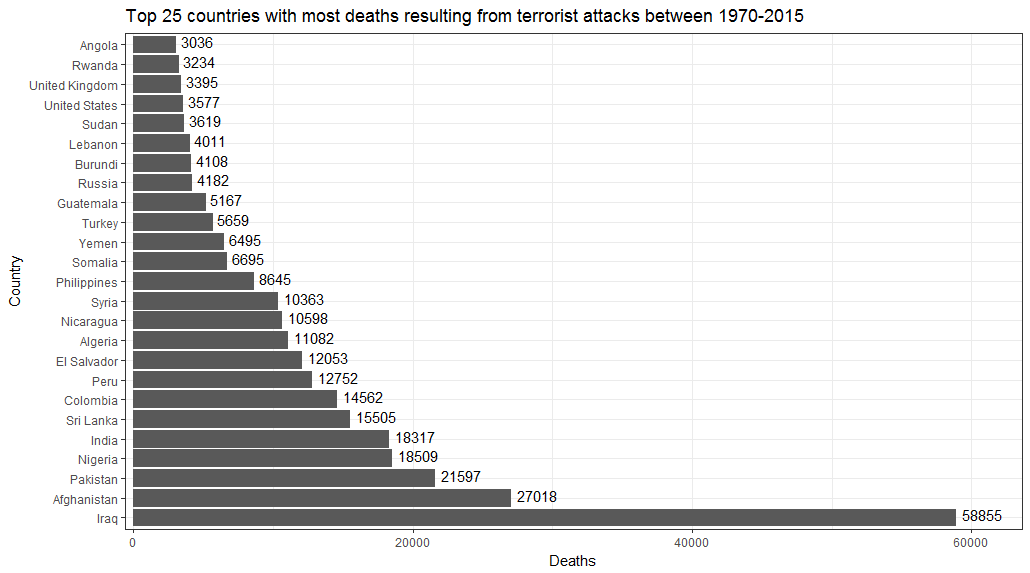
\includegraphics[width=0.8\textwidth]{Plots/Top25countriesbydeaths.png}
	\caption{Top 25 countries by number of deaths resulting from terrorism.}
\end{figure}
\end{center}

\subsection{Terrorism coverage in the United States news data}

\begin{center}
\begin{figure}[H]
		
	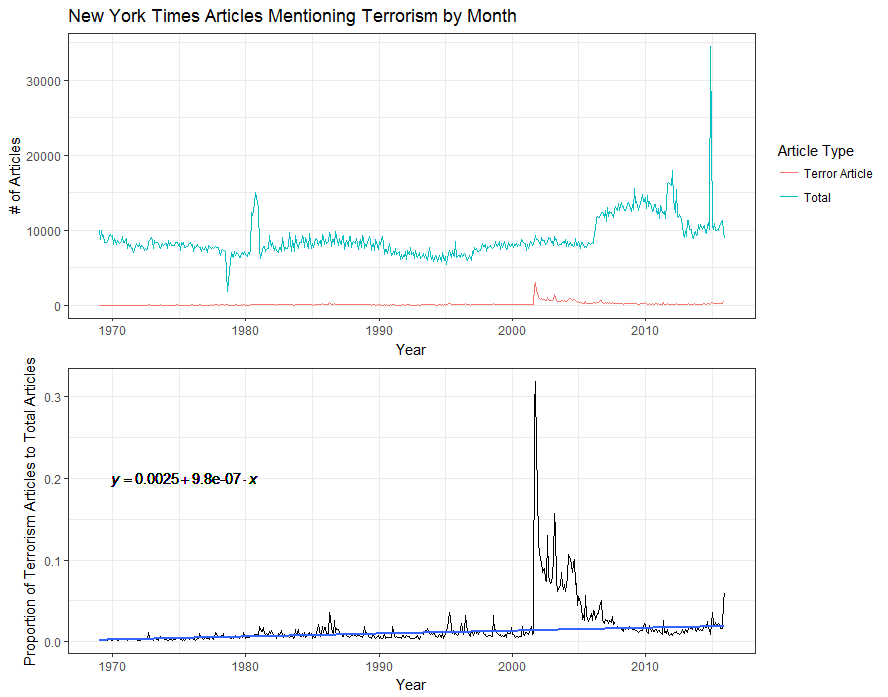
\includegraphics[width=0.8\textwidth]{Plots/NewsData/ArticlesByMonth.png}
	\caption{(Top) New York Times article count and terrorism article count by month. (Bottom) Proportion of terrorism related articles to total articles by month. This is fitted with a robust linear model in order to gain a general overview of possible temporal trends.}
\end{figure}

\begin{figure}[H]
	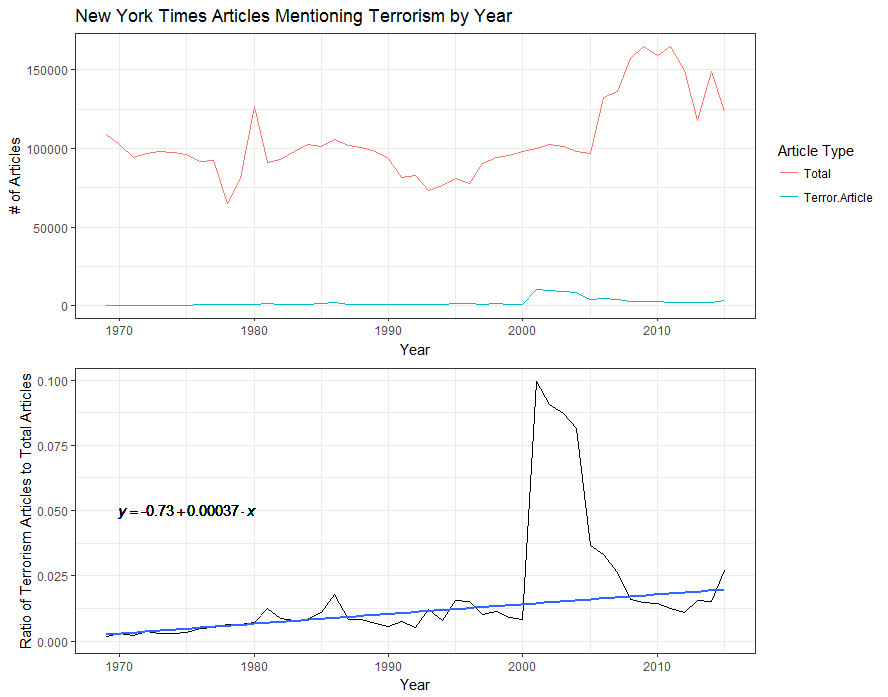
\includegraphics[width=0.8\textwidth]{Plots/NewsData/ArticlesByYear.png}
	\caption{(Top) New York Times article count and terrorism article count by year. 
	(Bottom) Proportion of terrorism related articles to total articles by year. This is fitted with a robust linear model in order to gain a general overview of possible temporal trends.}
\end{figure}

\begin{figure}[H]
	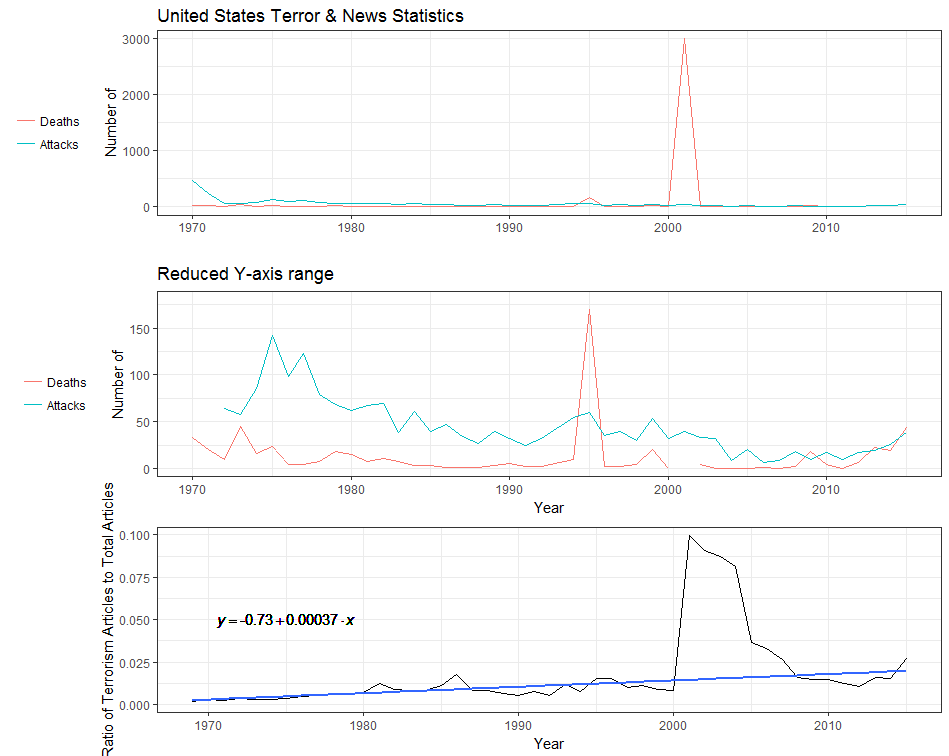
\includegraphics[width=0.8\textwidth]{Plots/NewsData/AttackNewsData.png}
	\caption{(Top) United states deaths and attacks due to terrorism by year. 
	(Middle) United states deaths and attacks due to terrorism by year with a reduced Y-axis range. 
	(Bottom) Proportion of terrorism related articles to total articles by year. This is fitted with a robust linear model in order to gain a general overview of possible temporal trends.}
\end{figure}
\end{center}

\subsection{Method of Attack}

\begin{center}
\begin{figure}[H]
	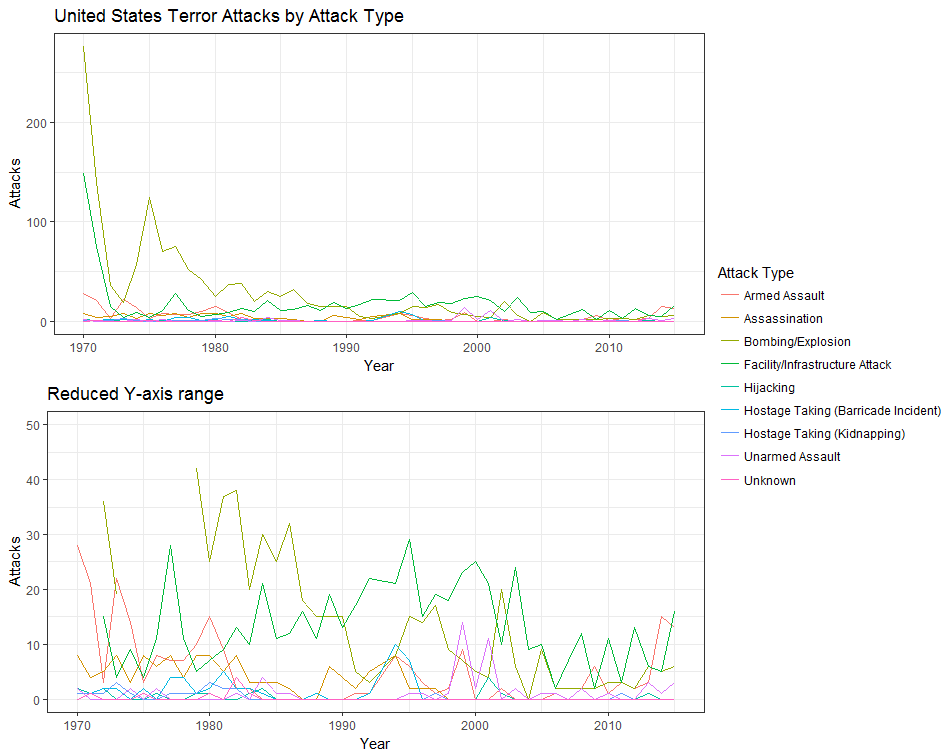
\includegraphics[width=0.8\textwidth]{Plots/AttackType/Attacks.png}
	\caption{United States terror Attacks by Attack Type by year.}
\end{figure}

\begin{figure}[H]
	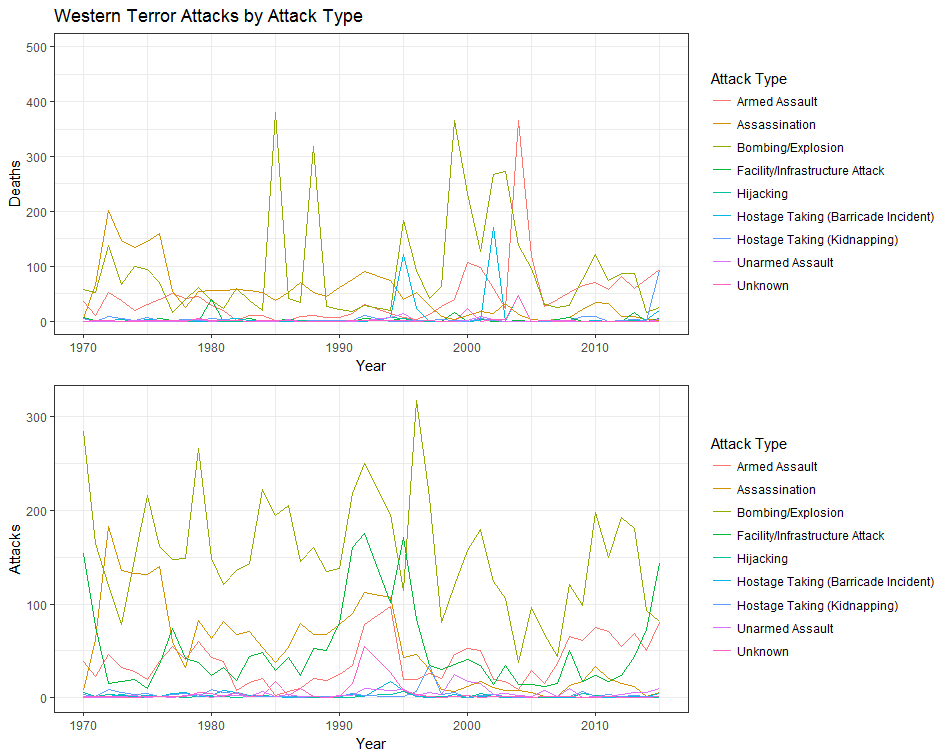
\includegraphics[width=0.8\textwidth]{Plots/AttackType/AttackTypeWesternCountries.png}
	\caption{Western Terror Attacks by Attack Type by year.}
\end{figure}

\begin{figure}[H]
	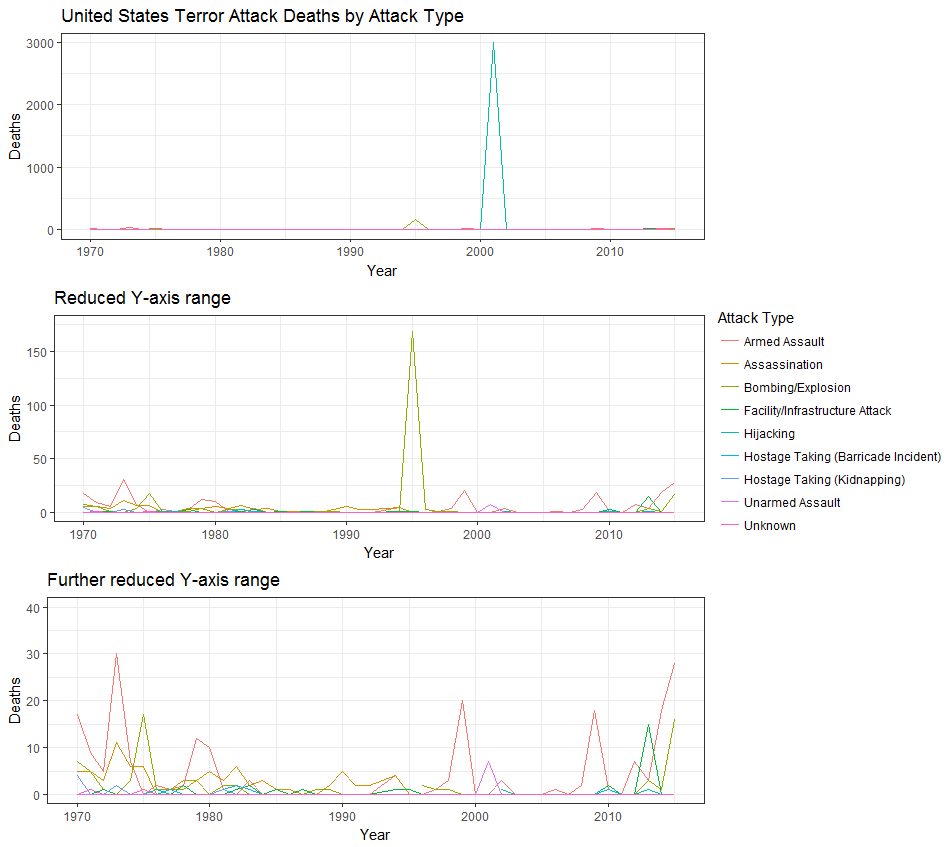
\includegraphics[width=0.8\textwidth]{Plots/AttackType/Deaths.png}
	\caption{United States terror Attack Deaths by Attack Type by year.}
\end{figure}

\begin{figure}[H]
	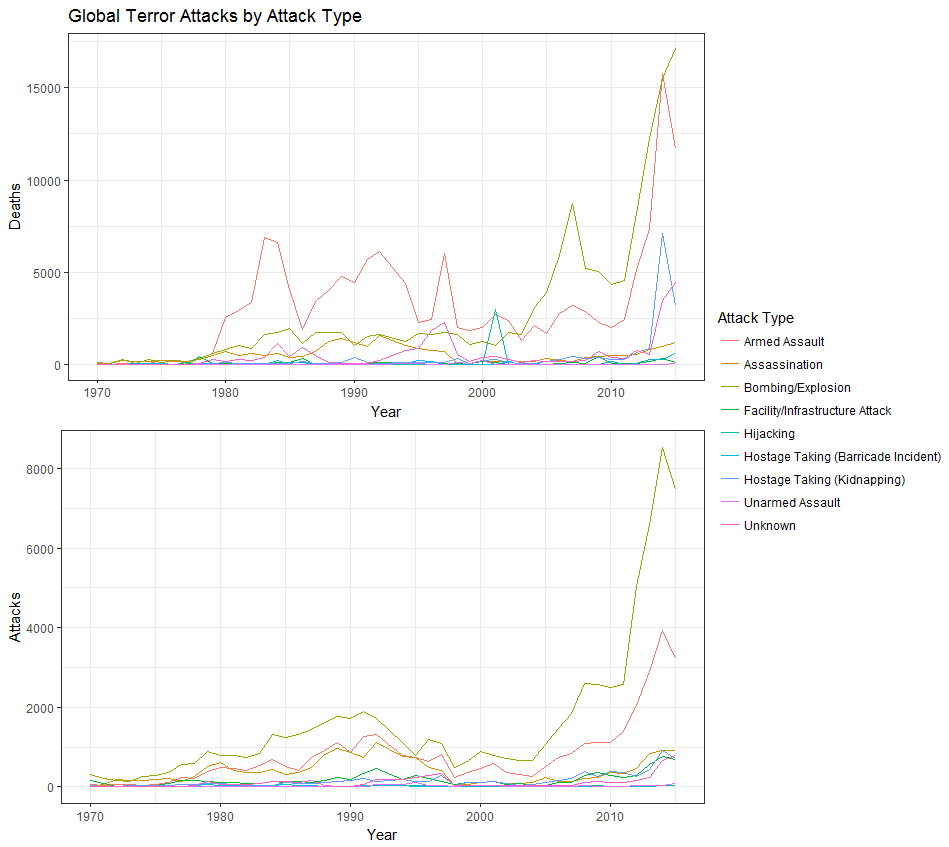
\includegraphics[width=0.8\textwidth]{Plots/AttackType/Global.png}
	\caption{Global Terror Attacks by Attack Type by year.}
\end{figure}

\begin{figure}[H]
	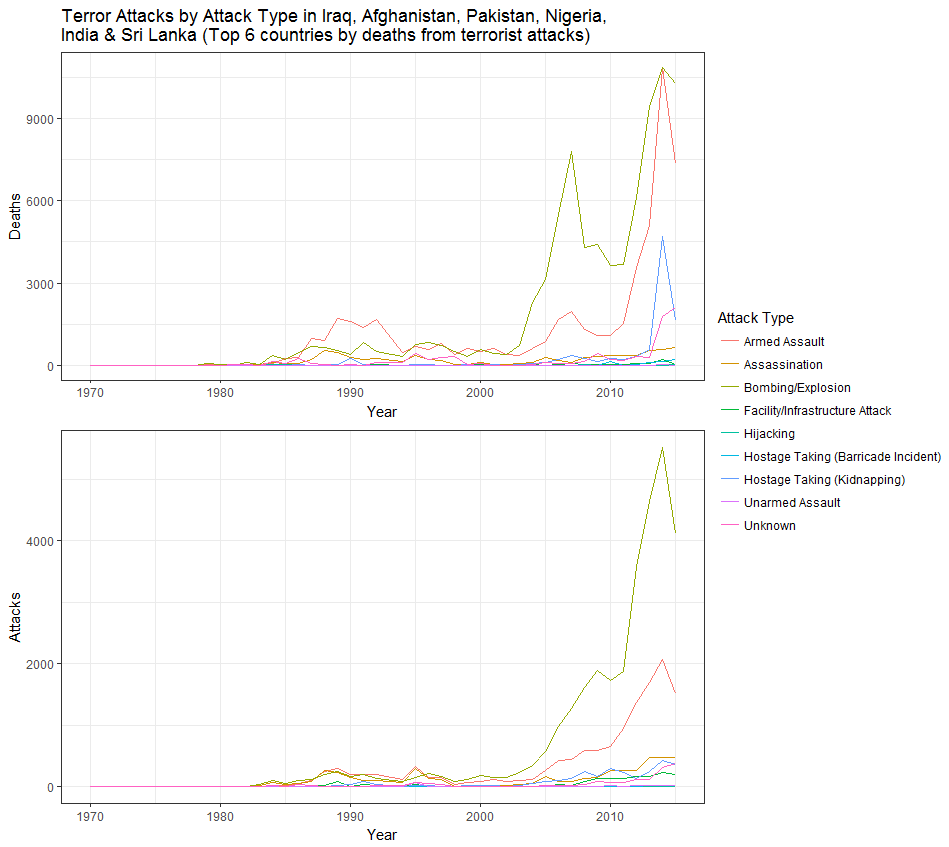
\includegraphics[width=0.8\textwidth]{Plots/AttackType/Top6.png}
	\caption{Terror Attacks by Attack Type in the top six countries by terrorism related deaths (Iraq, Afghanistan, Pakistan, Nigeria, India \& Sri Lanka).}
\end{figure}
\end{center}

\subsection{Terrorism trends over time}
\begin{center}
\begin{figure}[H]
		
	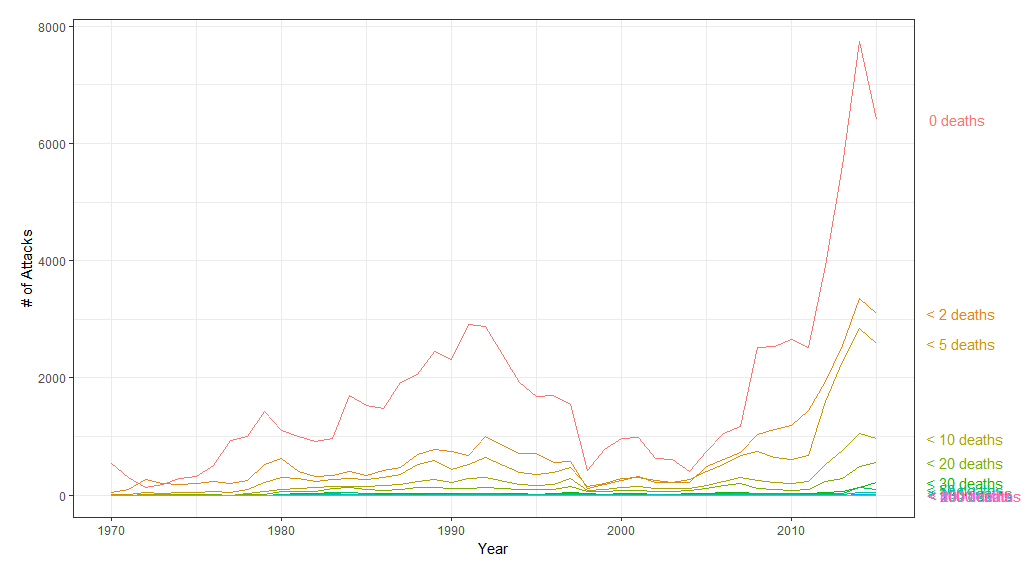
\includegraphics[width=0.8\textwidth]{Plots/OverTime/Attacks_over_time_grouped_by_deaths.png}
	\caption{Number of attacks by year grouped by the number of deaths resulting from the attack.}

\end{figure}
\end{center}

\subsection{Rates of success in terrorist attacks}
\begin{center}
	
\begin{figure}[H]
	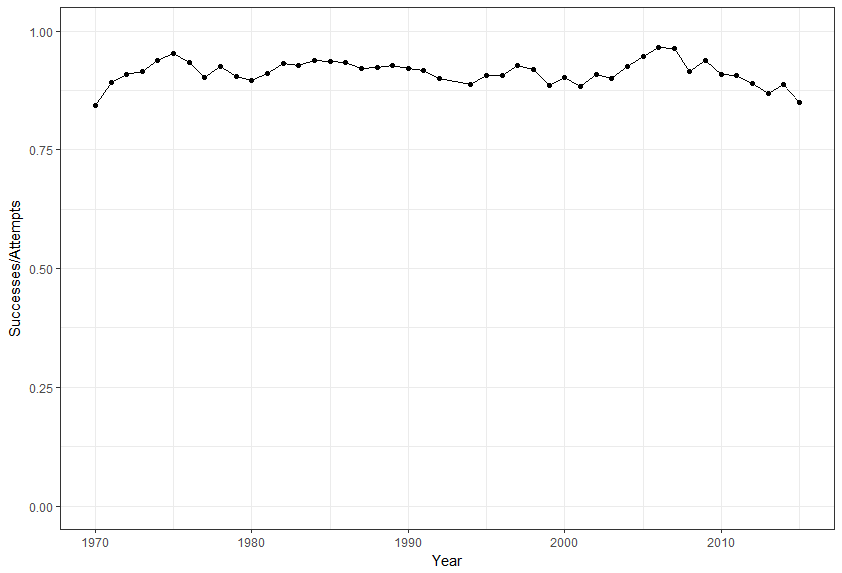
\includegraphics[width=0.8\textwidth]{Plots/OverTime/Successes_vs_Attempts_by_Year.png}
	\caption{Plot of ratio of successful terrorist attacks to total number of attacks globally.}
\end{figure}

\begin{figure}[H]
	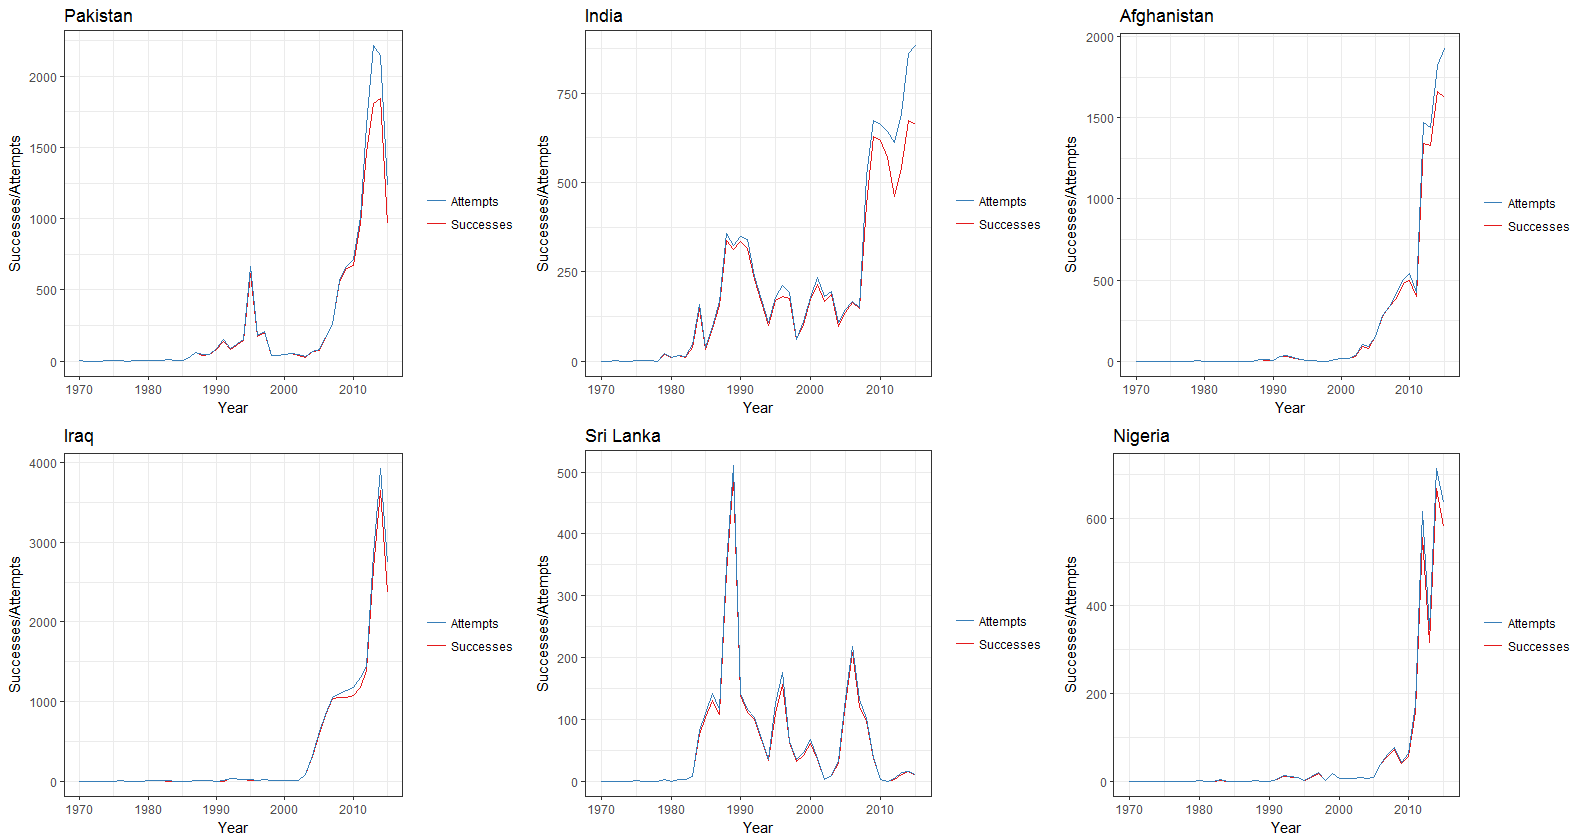
\includegraphics[width=0.8\textwidth]{Plots/OverTime/Top6SuccessVsAttempts.png}
	\caption{Number of successful and total number of attempts plotted by value by year for the Top 6 countries by total deaths as a result of terrorism.}
\end{figure}

\begin{figure}[H]
	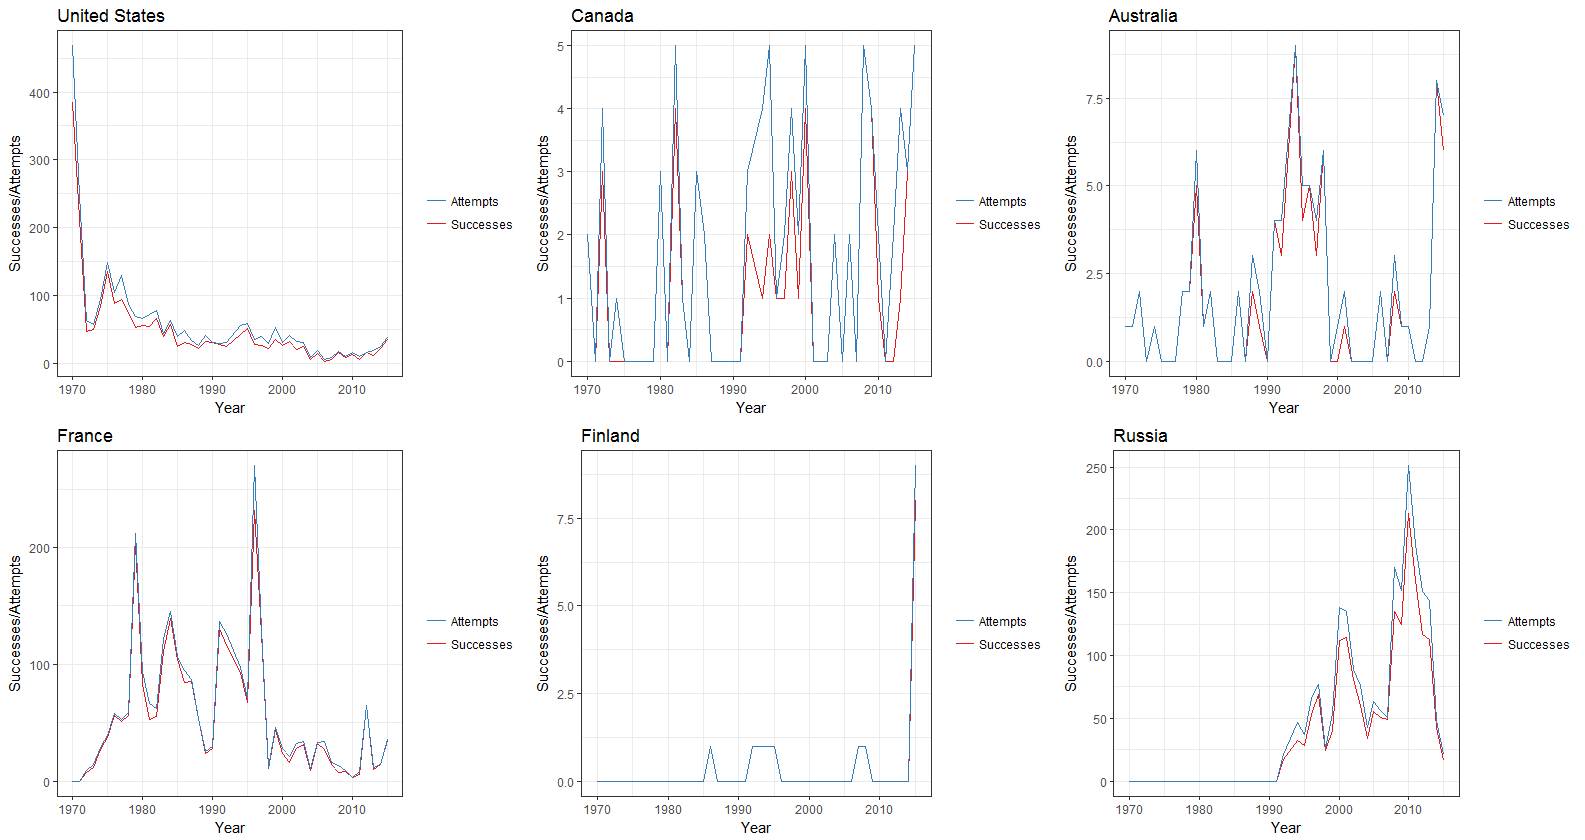
\includegraphics[width=0.8\textwidth]{Plots/OverTime/WesternSuccessVsAttempts.png}
	\caption{Number of successful and total number of attempts plotted by value by year for the six western countries: United states, Canada, Australia, France, Finland and Russia}
\end{figure}
	
\end{center}

\section{Discussion} 

\subsection{Terrorism coverage in United States news data}
The aim in this section is to Explore the relationship between Terrorist attacks, deaths and media coverage of attacks in the United States. In \textit{Figure 4}, the proportion of terrorism articles to total articles each month has a positive gradient robust linear regression, showing that through the 45 years from 1970 to the end of 2015, although very marginal (0.00037), more articles each month is being written about terrorism. From 1970 to September 2001 this linear regression is followed closely without much deviation but in in December, 2001, the month after \textit{911}, where there was a fatality count of \textit{2997} people, there is a large spike in terrorism articles, where the ratio peaked \textit{0.318667236}. In the following years after this attack the ratio slowly decreased until it settled onto the robust linear regression line, following it again.
\\\\
Further, when looking at \textit{Figure 6}, it can be seen that in Unites States, since 1970, while the ratio of terrorism articles to total articles is increasing, the number of attacks and deaths are decreasing. There could be multiple reasons why this is inversely proportional relationship between the ratio of articles and death/attack count such as the media following stories that would interest there readers due to a scare facto, the media being able to access more people through the uprise of the technology, expanding their target audience past people who read newspapers to everyone with an electronic devise, there being more threats of attacks but no actual attacks, there being a positive feedback loop between all of the news companies who are reporting of terrorism actions or America having more involvement. These reasons are all ideas though and have no statistical evidence, more data and time would be required to research this.
\\\\
When looking at the recent time, from 2012 to 2015, there has been a gradual increase in attacks and deaths, that is also represented in the increase in the media. Attacks and the article ration having a correlation of 0.38 and deaths and article ratio having a correlation of 0.41. This shows that the deaths, attacks and the number of articles related to terrorism are linked.
\\\\ 
From all of the data collected from the New York Times archives and being compared to the STAR terrorism archives, It is evident that there is a relationship between attacks, deaths and the ratio of terrorism articles to number of articles although there is a marginal increase in the ratio through the 45 years that is captured by START. This is seen in \textit{911, September 2001} where the deaths spiked and so did the article ratio, and from 2012 to 2015 there is a similar increase in deaths and articles.



\subsection{Methods of Attack}
In this section we explore the the hidden trends in methods of terrorism attacks. Looking at \textit{Figure 10}, there is a great increase in bombing/explosion and armed assault for both death count and attack count but in further analysis, it is seen that the way to view this trend is not globally, but by looking at it in regions due to some regions skewing the results and there being very different patterns through all of the different regions.
\\\\
In \textit{8}, the western countries although looking very erratic have a close to consistent ratio of different attack types from 1970 to 2015 for both death count and attack counts. This erratic nature of the graph is uninteresting and not minimal can be interpreted from it. When this is contrasted to \textit{Figure 11}, the 6 countries with highest deaths from terrorist attacks, it is evident that they are not similar at all.
\\\\
In the Top six countries bombing/Explosion and armed assault significantly increased from 2000 in the death and attack count, and Hostage Taking and unknown increasing from the 2003, largely contributing to the death count. This new uprise in terrorism related deaths is huge and could be related to a lot of reasons, such as poverty and war-torn city’s creating extremists coupled with new ways to find and recruit extremists and then organise and carry out the attacks due to the rise in technology and the new accessibility of instant free messaging and chat rooms, making it a lot easier to conduct such activities. These are just speculations though and more research will have to be done to prove/disprove them.
\\\\
\textit{Further looking at figure united stated terror attacks by attack type}, the amount of attacks and type of attacks have been decreasing since 1970. In \textit{9}, excluding the outlier \textit{911 in September 2001}, the amount of deaths are also low with armed assault, bombing/Explosion, and facility/infrastructure attack being the highest (27).
\\\
All around the world, each region follows a different rend line with the western countries having an erratic trend, showing minimal information, The top 6 countries with the highest terrorism related death toll having a very large increase deaths and America, whose attacks decreased. In general, armed assault, bombing/explosion, hijacking and hostage have increase over the years throughout all of the countries, resulting in them being the deadliest terrorist attack types.

\subsection{Terrorism trends over time}

Terrorism trends over time with regard to number of deaths as well as geographical trend visualisations have been conducted in depth in a number of investigations. 
As a result this section of the investigation comprises a small portion of the overall analysis. 
One aspect of the data that was explored was the trends in attacks by the number of deaths as a result of a given attack.
\\\\
The data shown in \textit{Figure 12} shows the number of attacks over time grouped by the number of people killed globally. 
This plot however does not accurately represent the number of people killed over the same time period, since this only looks at numbers of attacks of a certain magnitude in comparison to the number of deaths in total over some time period.
Additionally this does not take into account the number of injuries as a result of these attacks. 
Despite this, we notice a distinct trend. 
\\\\
The majority of attacks over the entire time period are attacks where nobody dies. 
With a total of 70947 attacks (53.02\%) with no deaths over the entire time period surpassing the number of attacks with only one death, which respectively comprised 27988 attacks (20.91\%).
Overall 88\% of attacks result in less than 5 deaths. 
97\% of all attacks result in less than 20 deaths.
The mean number of deaths per attack globally is 2.36. 
Ultimately, despite the greatly increasing number of attacks on a global scale, the number of deaths per attack is small. 
Since the GTD also classifies attacks on infrastructure as an attack, where nobody dies.
Looking only at attacks where one or more people die, we see the mean deaths per attack  increase to 4.92, more than double.
\\\\

\subsection{Rates of success in terrorist attacks}
As shown in the \textit{Figure 13}, the rates of success of terrorist attacks do not vary greatly on a global scale. Despite a greatly varying number of attacks and deaths, especially between the two main country clusters investigated (western countries and the top six countries with regard to total deaths as a result of terrorism), countries in these two clusters have very similar rates of success over time. 


\subsubsection{Westernised Countries}
For a sample of 6 western countries: United States, Canada, Australia, France, Finland and Russia; the respective mean success rates over the period of time 1970-2015 are 0.807, 0.725, 0.869, 0.904, 0.984 and 0.828; an overall mean success rate of 0.853. However these means misrepresent the number of successes and failures comparatively. Finland, with the highest success rate of the six western countries shown, however over the given time period, has had a total of 15 terrorist attacks, 14 of which were successful. 

Five of the six countries have had years during this period with no terrorist attacks, Canada: 20, Australia: 17, France: 2, Finland: 38, Russia: 22. The United States however, with a comparatively lower mean success rate, has had no years without a terrorist attack. The rate of success in the United States, despite counter-terrorism related government funding having doubled between 2001 and 2013 (Desilver, 2013).
\\\\
Other westernised countries specified above however, due to the low number terrorist attacks year to year, show very erratic rates of success over the time period.
In part this is visible in countries such as Finland and Australia where the overall number of attacks is low, and as such the success rate for years when there are no attacks are difficult to handle.
For this analysis, additionally for the further analysis of success rates for the \textit{Top 6}, years with one or more attack are often considered in determining mean values. 
\\\\
The highest number of attacks for each country in any given year: Australia, 9; Finland, 9; Canada, 5; United States, 468; France, 270; Russia, 251. The success rate for Australia, Finland and Canada becomes increasingly random, or in the case of Finland, increasingly high. However as seen in the United States, there is an overwhelmingly stable rate of success for terrorist attacks over the 45 year period. It must be noted that in all of the western countries shown in \textit{Figure 15}, the number of has decreased greatly among countries with previously high rates of attack (United States, France and Russia). As a result, we see erratic success rates for a small number of attacks in a given year. Despite this, it is evident in \textit{Figure 15} that the ratio of successful attacks to total attacks is comparatively high, with a mean of 0.853 as noted previously.
\\\\
In the six westernised countries investigated in \textit{Figure 15}, the number of attacks has decreased over the period of time in question with even recent years a decrease of attack attempts from 251 to 21 and successes from 213 to 16 between 2010 and 2015. With rate of success decreasing from 0.849 in 2010 to 0.762 in 2015. However this decrease, while being of great magnitude, due to the decreased number of attacks may be skewed. On the contrary in 2014, a success rate of 0.896 was observed. As a result, while the number of attacks is decreasing, it can be said that the rate of success for these attacks is not.
\\\\
While the rate of success for attacks in the west does not appear to be changing drastically in both recent years and over the entire relevant time period, the number of attacks in each of the six countries investigated has decreased drastically. Consequently the rate of success is skewed by the total number of attacks yet remains at a significantly high level.

\subsubsection{Top 6 Countries with respect to deaths from terrorist attacks}
The top six countries with respect to deaths from terrorist attacks are decided upon using \textit{Figure 3}, and are subsequently Iraq, Afghanistan, Pakistan, Nigeria, India and Sri Lanka. These countries will be referred to as simply the \textit{Top 6} for the remainder of this section.
\\\\
These countries, chosen for their comparatively high number of deaths due to terrorism, have higher mean success rates over the period of time between 1970 and 2015.
The data in \textit{Figure 14} shows the number of successful attacks as well as the number of total attacks by year for the countries within the \textit{Top 6}. With mean success rates of:
\\\\ 
\indent Pakistan: 0.939\\
\indent India: 0.918\\
\indent Afghanistan: 0.893\\
\indent Iraq: 0.907\\
\indent Sri Lanka: 0.936\\
\indent Nigeria: 0.932\\
\\
An overall mean success rate of 0.922, higher than that in the western countries mentioned by 0.069. The rate of success in these countries is approximately 0.07 higher than in western countries, however in 2010-2015 alone there were 36978 attacks and 32788 successes, an overall mean success rate of 0.887 over the five year period. In comparison to the mean success rate in western countries over the same time period, while a greatly decreased number of attacks and successes (1110 and 936 respectively), the success rate was 0.843. The difference in success rates of terrorist attacks in two vastly different groups of countries with respect to geographical location as well as number of deaths due to terrorist attacks, differs by only 0.044.
\\\\
As mentioned previously as part of the success rate analysis of western countries, the success rate can be skewed by a very low number of attacks. This can be observed for all of the Top 6 countries in the first portion of the time period shown. However for all of the Top 6, excluding Sri Lanka, in the most recent time period (2000-2015), the number of attacks has rapidly grown, with 36978 attacks and 32788 successes in that time period alone. With this massive increase in the number of attacks however, we see a convergence of success rates among almost all of the six countries. With the average success rate over the six countries reaching 0.835 in 2015, country specific success rates maintain high mean values over the five year period however we see at the peak number of attacks for a number of these countries, a drop in the success rate:
\\\\
\indent \indent(Country: five year mean, 2015 success rate - 2015 attack number) \\
\indent Pakistan: 0.873,  0.781 - 1235  \\
\indent India: 0.814, 0.750 - 882 \\
\indent Afghanistan: 0.909, 0.844 - 1926 \\
\indent Iraq: 0.918, 0.862 - 2743 \\
\indent Sri Lanka: 0.844, 0.818 - 11 \\
\indent Nigeria: 0.911, 0.912 - 637 \\
\\
While some of these countries show low rates of success in 2015 in comparison to their five year average such as Pakistan and India, it is key to note that the number of attacks as seen in \textit{Figure 14} is at an all time high.

\subsubsection{Conclusion}
Despite the large geographic difference between the \textit{Top 6} and the westernised countries investigated, there remains a very high success rate of terrorist attacks despite fluctuations in the number of attacks as a whole.
In those Western countries alone, we see a high rate of success with minor fluctuations in countries with an additionally large number of attacks such as the United States.
Countries with generally low numbers of terrorist attacks such as Finland and Australia, suffer from extremely high rates of success.
Regardless of the geographic location, the rate of success seems to be significant, and in the two geographic clusters, greater than 0.8 in all countries excluding Canada, which respectively has a mean success rate of 0.725.


\section{Further Work} 
Due to the exploratory nature of this investigation, there are numerous possibilities for future work.
From the conclusions reached in this investigation, further work in the area of deaths and attack rates by country controlled by population is a necessary step to further understand the data.
Two geographic clusters were investigated in this report:
\\\\
\indent Cluster 1 (Western Countries): United States, Canada, Australia, Finland, France and Russia. \\
\indent Cluster 2 (Top 6): Pakistan, India, Afghanistan, Iraq, Sri Lanka and Nigeria.
\\\\
While these clusters were used to determine differences between typically westernised countries and the top six countries with respect to deaths from terrorism, a well defined clustering of countries regarding the variables in this data should be investigated.


\pagebreak
\begin{thebibliography}{9}

\bibitem{1}
National Consortium for the Study of Terrorism and Responses to Terrorism (START). 
(2016). \textit{Global Terrorism Database}[Data file].
Retrieved from https://www.start.umd.edu/gtd

\bibitem{2}
Charters, D. (1989). Terrorism: A survey of recent literature. Conflict Quaterly, 64-84.

\bibitem{3}
Cornell Law. (n.d.). 18 U.S Code. Retrieved from https://www.law.cornell.edu/text/18/2331

\bibitem{4}
CPOST. (2016, June). The Chicago Project on Security and Terrorism. 
Retrieved from University of Chicago: http://cpost.uchicago.edu/

\bibitem{5}
DoD. (2010). DoD Dictionary of Military and Associated Terms. 
Retrieved from http://www.dtic.mil/doctrine/new\_pubs/dictionary.pdf

\bibitem{6}
FBI. (2002). Terrorism 2002 - 2005. 
Retrieved from https://www.fbi.gov/stats-services/publications/terrorism-2002-2005

\bibitem{7}
FEMA. (2013, July 25). Terrorism. 
Retrieved from FEMA.gov: https://www.fema.gov/media-library-data/20130726-1549-20490-0802/terrorism.pdf

\bibitem{8}
Hill, O. (2016). Contra Wars: The CIA and Its Own Definition of Terrorism. Crescast Scientia Journal of history, 55.

\bibitem{9}
LaFree, G. (2010). The Global Terrorism Database: Accomplishments and Challenges. 
Retrieved from Persepectives on Terrorism Vol 4, No 1: http://www.terrorismanalysts.com/pt/index.php/pot/article/view/89/html

\bibitem{10}
LaFree, G., \& Dugan, L. (2004). How does studying terrorism compare to studying crime? 
Retrieved from Terrorism and Counter-Terrorism (Sociology of Crime, Law and Deviance, Volume 5) Emerald Group Publishing Limited, pp.53 - 74: http://www.emeraldinsight.com/doi/pdfplus/10.1108/S1521-6136%282004%290000005006

\bibitem{11}
Lafree, G., \& Dugan, L. (2007). Introducing the Global Terrorism Database. 
Retrieved from Terrorism and Political Violence: https://ccjs.umd.edu/sites/ccjs.umd.edu/files/pubs/FTPV\_A\_224594.pdf

\bibitem{12}
LaFree, G., Dugan, L., \& Scott, J. (2006). Building a Global terrorism Database. 
Retrieved from University of Maryland: https://www.ncjrs.gov/pdffiles1/nij/grants/214260.pdf

\bibitem{13}
Legal Information Institute. (2016). 22 U.S Code. 
Retrieved from Cornell Law School: https://www.law.cornell.edu/uscode/text/22/2656f

\bibitem{14}
Merari, A. (2007, December 21). Academic research and government policy on terrorism. 
Retrieved from Terrorism and Political Violence: http://www.tandfonline.com/doi/abs/10.1080/09546559108427094

\bibitem{15}
Pape, R., Kevin, R., Bauer, V., \& Jenkins, G. (2014, August 11). How to fix the flaws in the Global Terrorism Database and why it matters. Retrieved from New York Times: 

\bibitem{16}
Desilver, D. (2013). \textit{U.S. spends over \$16 billion annually on counter-terrorism}.
Retrieved from http://www.pewresearch.org/fact-tank/2013/09/11/u-s-spends-over-16-billion-annually-on-counter-terrorism/

\end{thebibliography}

\end{document}
